\documentclass{standalone}
\usepackage{pgf, tikz}

\usetikzlibrary{arrows, automata}

\begin{document}

    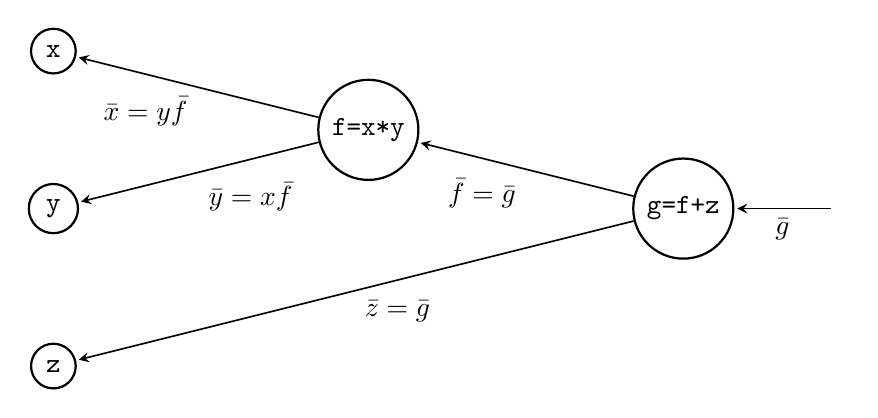
\begin{tikzpicture}[
            > = stealth, % arrow head style
            shorten > = 1pt, % don't touch arrow head to node
            auto,
            node distance = 3cm, % distance between nodes
            semithick % line style
        ]

        \tikzstyle{every state}=[
            draw = black,
            thick,
            fill = white,
            minimum size = 4mm
        ]

        \node (x) [state] at (0,0) {\texttt{x}};
        \node (y) [state] at (0,-2) {\texttt{y}}; 
        \node (z) [state] at (0,-4) {\texttt{z}};  
        \node (f) [state] at (4,-1) {\texttt{f=x*y}};
        \node (g) [state] at (8,-2) {\texttt{g=f+z}};
        \node (out) at (10,-2) {};
        
        \path[->] (f) edge node {$\bar{x} = y\bar{f}$} (x);
        \path[->] (f) edge node {$\bar{y} = x\bar{f}$} (y);
        \path[->] (g) edge node {$\bar{f} = \bar{g}$} (f);
        \path[->] (g) edge node {$\bar{z} = \bar{g}$} (z);
        \path[->] (out) edge node {$\bar{g}$} (g); 

    \end{tikzpicture}

\end{document}
